\chapter{Definitions, Features, and Abbreviations Used}
\label{Kapitel Begriffe} 

	\minisec{Unit}
...see teaching unit.
	
	\minisec{Department}
...see Institute.

	\minisec{Institute}
An institute is the entity responsible for allocating lecturers for the individual degree programs and subjects.
An example is the "`Languages"' Institute, which is responsible for all language-related subjects. (English, French, Japanese,...)

	{\minisec{Schedule Conflicts}
TEMPUS\raisebox{1ex}{\tiny\copyright} 2.0 checks the availability of lecturers, students and rooms as well as the times lecturers have marked as unavailable and reservations when making entries or changes to the teaching schedule. Should there be a scheduling conflict with one of the three schedules, an error message will appear and the action will be cancelled.
However, a conflict can be forced by disabling the conflict check in the "'Settings"' menu. The conflict check should always be enabled again afterwards, as otherwise this could easily lead to errors in the scheduling. (see chapter \ref{Kapitel Kollisionen})

	\minisec{KW...Calendar Week}
The year consists of at least 52 numbered calendar weeks (CW). According to DIN 1355 / ISO 8601, the first week of the year is the week in which at least four days fall in the new year. 

	\minisec{University Council}
The University Council consists of all the program directors, teacher representatives, heads of the departments and students, and is responsible for making all important strategic decisions for the UAS Technikum Wien.
	
	\minisec{LE...Teaching Unit}
The teaching unit contains all the essential, variable data needed to carry out the schedule planning. The data in the teaching units is used specifically for planning the teaching schedule and also as a source for the CIS page. Teaching assignments are also created based on this data. 

The teaching unit brings lecturers, students, subjects, etc. together and must be revised each semester.

See chapter \ref{Kapitel Lehreinheiten} for a detailed description.

For comparison, see "'LV...Course"'

	\minisec{Teaching Unit\_ID}
The teaching unit\_ID is a unique internal number that is assigned to each teaching unit.
Most tables in the database are linked to the teaching unit\_ID

	\minisec{Subject}
A subject determines the content of a teaching unit. (e.g., mathematics)

It defines the department responsible, the color (which is displayed in the teaching schedule), and the language of instruction. A subject is created for each degree program and each corresponding semester. The abbreviation for the subject is displayed together with the course type at the top of the teaching schedule. 
The course type for the classroom instruction (exercise, lecture, ILV,...) is, however, not defined here.

	{\minisec{Course Type}
The course type describes the subject in more detail in that it specifies the type of teaching that will take place. 

A course type can be a lecture (-VO) for example. This describes frontal teaching without independent practice. 

Other examples include exercise (-UE), integrative course (-ILV), lab sessions (-LAB) or tutorials (-TUT)

	\minisec{Teaching Schedule (=Timetable)}
The teaching schedule is the surface on which the teaching units are graphically displayed in color with the lecturers, the teaching groups and the rooms. 

It is possible to browse through the rooms and course weeks in the teaching schedule and it can also be exported from here for various other applications.

	\minisec{Teaching Group}
The teaching group refers to the organization of students into degree program, semester, divisions and groups. 

It serves to organize and divide larger numbers of students to create smaller groups for a better overview. 

An example at the UAS Technikum Wien would be: BEL-2A1. (Bachelor's Degree Program Electronics, 2nd Semester, Division A, Group 1) 

	\minisec{LFVT...Degree Program Course Schedule}
The degree program course schedule is the complete list of all teaching units that are to be planned for a semester of a degree program.

	\minisec{LV...Course}
A course is understood in the overall system the same as it is in the application of the degree program. It contains the basic master data. In contrast to the teaching unit, the course contains data that generally remain unchanged from year to year. It forms the basic foundation upon which all other tables are built.\\
The course is always seen from the perspective of a degree program or from the perspective of the student. The title of the course can be found on the transcripts and in the Teaching section on the CIS page. The course is not to be confused with the subject or the teaching unit (see individual definitions).\\
Courses that have been used once can no longer be removed but only disabled because otherwise the student grades for the course would be lost.

Attributes of the course are, for example, the abbreviation, the degree program, the semester in which it is taught, the language, the ECTS credits or the semester hours.

	\minisec{Module, Special Groups}
In addition to the regular teaching groups, there are modules and special groups which may contain different students.
It is thus possible to create groups of students from different teaching groups within a semester, or even from different semesters or degree programs. However, since special groups make it significantly more difficult to check for schedule conflicts and produce a teaching schedule without errors, special groups should be avoided as far as possible.

	\minisec{Infotip}
An infotip appears when the user holds the mouse over an element for a short time without clicking.

	\minisec{Room Type}
The attribute "'Room Type"' is used to summarize the various classrooms.
For example, a room type might be "'seminar room"'. This combines any number of single rooms into a whole.
The attribute is mainly used to obtain a clear number of suggested rooms for a teaching unit when planning the teaching schedule.

	\minisec{Reservation}
The teaching plan allows lecturers and staff to reserve a room in order to ensure they have a room available in the medium term and to keep the room from being used for the teaching schedule or by other teachers and staff.
It is only possible to reserve a room within a predefined time frame. Any reservation that has been made generally has precedence over regular teaching.

In practice, this may sometimes prove extremely inconvenient. Often external events, guest lectures, parties and graduation ceremonies are the reason for inconvenient changes to the room allocations. However, these irregular events are an important part of the University's day to day business, so it is not likely that a more convenient solution will be found other than giving priority to such events.

	\minisec{Semester (Year)}
A semester (from Latin: sex=six; mensis=month) is half of an academic year at a university. This also includes the semester break (= time in which there are no lessons).
As a rule, odd semesters (1,3,5,...) are in the winter semester (from September to February) and even semesters (2,4,6,...) are in the summer semester (from March to August) 

	\minisec{Special Groups}
...see Modules

	\minisec{Degree Program}
A degree program is the learning content offered at a university that culminates in the award of an academic degree. 

The curriculum of a degree program is defined by the study regulations and the examination results and the completion of the degree program are defined by the examination regulations. 

A degree program is concluded with the awarding of an academic degree such as a Bachelor's, or Master's degree.

	\minisec{Study Semester}
The study semester is a unique designation for a semester and a calendar year.
Accordingly, "'WS2007"' is the winter semester in 2007.

	\minisec{Blocking of Teaching Units}
The blocking of teaching units indicates how many units should be scheduled at a time (i.e. in direct succession). Since a single unit (for units of 45 minutes) is often inadequate, the blocking of teaching units will in most cases be at least "'2"'.

	\minisec{Timetable}
...see Teaching Schedule

	\minisec{UNR...Teaching Unit Number}
The teaching unit number is a sequential number that is automatically generated by the system and is relevant mainly for background processes. Normally, the UNR is the same as the teaching unit\_ID. 
It is important to note that the conflict check for the teaching schedule is based on the UNR. Teaching units with the same UNR can therefore be scheduled parallel to each other without causing an error.

	\minisec{Unit}
A day can be divided into any desired number of units with a starting and an ending time. However, the starting times may not overlap.
For example, at the UAS Technikum Wien, the day is divided into 16 units of 45 minutes each starting at 8:00 a.m.

	\minisec{Weekly Rhythm}
If a course is held at regular intervals throughout the semester, the interval can be specified in the attribute "'Weekly Rhythm"'.
A weekly rhythm of "'2"' therefore means that the course should take place every 2 weeks.

	\minisec{Unavailable Time}
"'Unavailable Time"' is an extension of the "'Preferred Teaching Time"' feature designed to obtain detailed information about the availability of a lecturer.
It is thus possible for the lecturer to mark an unlimited amount of specific dates as unavailable (for example, due to conferences, stays abroad, vacation or training). An unavailable time is highlighted in the LV-Plan in dark-red and an error will occur should anything be scheduled for this time. (see chapter \ref{Kapitel Kollisionen})

	\minisec{Preferred Teaching Time}
In their profile, each lecturer is able enter their preferred teaching time based on a normal week grid. The lecturer can assign values from -2 to +2 for every day and every unit in a week to indicate their availability. This pattern is then applied for all the weeks of a semester.
The preferred teaching times should be chosen according to the fair play principle, so that at least three times as many teaching units are assigned a positive value as are to be taught according to the teaching assignment.

\begin{tabular}{rll}
+2&...&I would like to teach at this time\\
+1&...&I can teach at this time\\
-1&...&I can only teach at this time in emergencies\\
-2&...&I can not teach at this time\\
\end{tabular}

The values are shown in the background according to a color system (from red to green). The default is +1. 

Practice shows that the lecturers often do not take advantage of this feature or have such limited flexibility that it is not possible to plan a teaching schedule without problems. In some cases, even fewer teaching units are assigned a positive value than the lecturer is actually supposed to teach each week.
Furthermore, the preferred teaching times are rarely updated, which in turn leads to subsequent changes.
For this reason a disciplined use of the preferred teaching times is an essential basis for effectively planning the teaching schedule.

The TEMPUS\raisebox{1ex}{\tiny\copyright} program indicates the preferred teaching time with a background color when selecting a lecturer or setting a teaching unit.

\begin{figure}
	\centering
	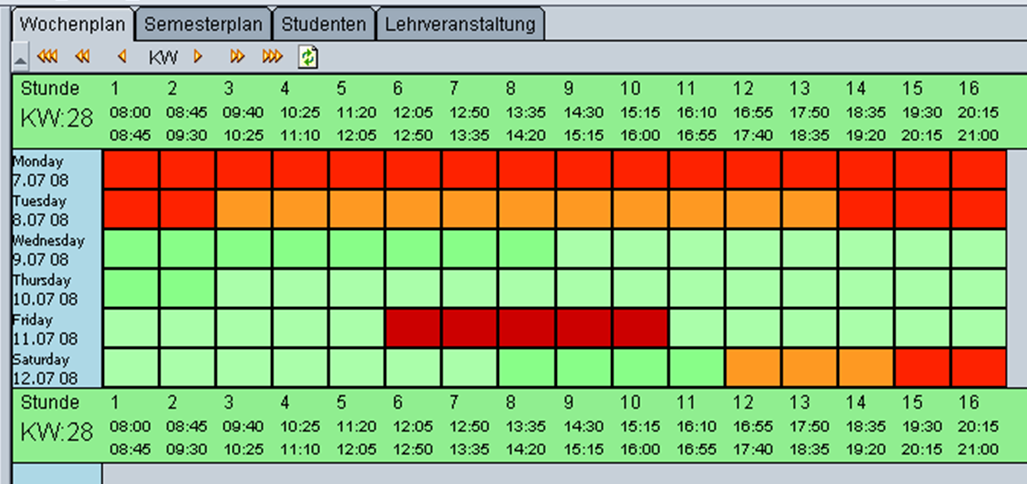
\includegraphics[width=0.8\textwidth]{Tempus_Beispiel_Zeitwunsch}
	\caption{Example of a preferred teaching time with all four values and a time on Friday marked as unavailable (dark red)}
	\label{Zeitwunsch}
\end{figure}
